\thislesson{19 Settembre 2016}{Introduzione, Parte prima}

In questo corso studieremo le funzioni meromorfe periodiche, ovvero $f:\bbC\to\bbC$ per le quali $f(z+T)=f(z)$ per ogni $T\in L$, con $L$ insieme dei periodi.\\
Partiamo dalle funzioni con un solo periodo, ovvero a meno di rinormalizzazioni consideriamo $L=\bbZ$.  Osserviamo che $f$ può passare al quoziente, ovvero posso definire $\tilde f:\bbC / \bbZ\to\bbC$ in modo che $\tilde f(x+\bbZ)=f(x)$. Lo spazio topologico quoziente $\bbC / \bbZ$ (ovvero $\bbC$ quozientato per la relazione di equivalenza $a \cR b \sse a-b \in \bbZ$) è un cilindro (in particolare notiamo che non è compatto).\\
Questo esempio ci dà molti spunti interessanti, e cercheremo di estenderlo introducendo il concetto di reticolo.\\

\section{Reticoli}
Il fatto che nell'esempio abbiamo preso $L=\bbZ$, che è un gruppo, non è un caso. Vale infatti
\begin{lemma}
  Sia $f: \bbC \rar \bbC$ una funzione meromorfa non costante.  Allora valgono:
  \begin{enumerate}
      \item l'insieme $L_f$ dei periodi di $f$ forma un sottogruppo additivo di $\bbC$.
      \item $L_f$ è discreto
      \item $L_f$ può essere isomorfo solo al gruppo banale, a $\bbZ$ o a $\bbZ^2$
  \end{enumerate}
\end{lemma}
\begin{proof}
      Consideriamo $\alpha,\beta\in L_f$ ovvero tali che $f(z + \alpha) = f(z)$ e $f(z + \beta) = f(z)$ $\forall z$; si ha allora facilmente $f((z + \alpha) + \beta) = f(z + \alpha) = f(z)$, ovvero $\alpha+\beta\in L_f$. Inoltre banalmente $0\in L_f$, e si vede che anche $-\alpha\in L_f$, poiché $f(z)=f((z-\alpha)+\alpha)=f(z-\alpha)$.\\
      Vogliamo ora dimostrare che se $L_f$ è denso in $\bbC$, allora $X=\bbC / L_f$ è banale, ovvero $f$ sarebe costante. Consideriamo un aperto $U\subset X$ non vuoto; per definizione di quoziente, $\pi^{-1}(U)=V$ è un aperto di $\bbC$, e vale $V+g=V\forall g\in L_f$. Prendiamo uno $z\in\bbC$ e consideriamo il traslato $V-z$, che è ancora un aperto di $\bbC$; dato che $L_f$ è denso, esisterà un $t\in L_f\cap (V-z)$. Ma allora $z\in V-t=V$, cioè dato che $z$ era generico, $V=\bbC$ e dunque l'unico aperto non vuoto del quoziente è l'intero spazio.\\
      L'ultimo punto lo mostreremo più avanti.
\end{proof}

D'ora in poi il gruppo $L_f$ dei periodi lo chiameremo \emph{reticolo} di $f$, motivati anche dalla
\begin{definizione}[Reticolo]
  Un \emph{reticolo} è un insieme parzialmente ordinato in cui ogni coppia di elementi ha sia un estremo inferiore che un estremo superiore. La relazione d'ordine su $L_f$ è quella data dal modulo(?).
\end{definizione}

Consideriamo ora $L_f \cong \bbZ^2$: possiamo descrivere $L_f = \omega_1 \bbZ + \omega_2 \bbZ$ con $\Img \frac{\omega_1}{\omega_2} \neq 0$, e questo tipo di reticolo ci accompagnerà per tutto il corso, in quanto

\begin{definizione}[Funzione ellittica]
  Una funzione $f$ si dice ellittica se il suo reticolo dei periodi $L_f$ ha rango $2$.
\end{definizione}

\begin{osservazione}
  Se $L_f$ ha rango 2, $\bbC / L_f$ è omeomorfo ad un toro, quindi le nostre funzioni ellittiche le possiamo anche pensare come funzioni olomorfe definite da un toro (come varietà olomorfa) a $\bbC$. Ricordiamo che il toro è compatto.\\
  Inoltre esiste sempre un dominio fondamentale, che è dato dal parallelogramma di vertici $0,\omega_1,\omega_2,\omega_1+\omega_2$, identificando i bordi
\end{osservazione}

Il fatto che il toro sia compatto implica che non esistono funzioni ellittiche olomorfe: se infatti $f$ è ellittica e olomorfa, esiste un punto del parallelogramma fondamentale in cui $|f|$ ha massimo; ma essendo $f$ intera e limitata, deve essere costante per il teorema di Liouville.\\
Vediamo invece che su $\bbR^2$ esistono funzioni regolari con gruppo di periodi $G$ di rango $2$:
\notamargine{La regolarità nei complessi è molto più forte che non nei reali. Essere olomorfe è davvero tanta roba in più che non essere $C^\infty$}
\\
Basta prendere una $\varphi:\bbR^2\to\bbR$ liscia a supporto compatto, e definire $\psi(x)=\sum_{g\in G}\varphi(x+g)$ (è una somma finita poiché $\varphi$ è a supporto compatto). Chiaramente $\psi$ ha gruppo di periodi uguale a $G$.

D'altra parte abbiamo una descrizione completa delle funzioni olomorfe con periodi di rango $1$:
\begin{esercizio}
  Le funzioni olomorfe con periodo $z_0$ sono tutte e sole quelle della
  forma $z \mapsto g(e^{2\pi i z/z_0})$, con $g$ funzione olomorfa.
\end{esercizio}

Per andare avanti ci servirà introdurre il concetto di varietà complessa, o superficie di Riemann:
\begin{definizione}[Superficie di Riemann]
  Si dice una superficie di Riemann una varietà complessa connessa di dimensione $1$.  Si intende che ogni punto deve avere un intorno $U_\alpha$ omeomorfo al disco unitario aperto di $\bbC$ tramite l'omeomorfismo $\phi_\alpha$, e che per ogni $\alpha$ e $\beta$ valga che $g := \phi_\beta \circ \phi_\alpha^{-1}$ sia una funzione olomorfa.
\end{definizione}

\begin{esempio}
  $\bbC / \bbZ$ è una superficie di Riemann, ma non è omeomorfa a $\bbC$ (Ad esempio perché $\bbC$ è semplicemente connesso, mentre $\bbC / \bbZ$ non lo è).
\end{esempio}

\paragraph{Definizione della struttura olomorfa dei tori}
Preso un parallelogramma fondamentale del reticolo, possiamo considerare come aperti gli aperti di $\bbC$ che non toccano due punti equivalenti e considerando la mappa di immersione degli stessi in $\bbC$ si ottiene la struttura di Superficie di Riemann del Toro.
\notamargine{Tutti i reticoli di rango $2$ sono isomorfi come gruppi, ma la struttura olomorfa che inducono sui tori quoziente è molto diversa}


\paragraph{Curiosità - Delirio}
% DOUBT: Non sono davvero sicuro che alludesse a Chow, ma mi pare quello che ci sta di più
È molto importante che i Tori siano compatti, poiché le superfici di Riemann compatte sono descritte da equazioni algebriche (Forse fa riferimento al teorema di Chow)


\section{Curve ellittiche}
Andiamo ora ad introdurre l'oggetto algebrico strettamente legato alle funzioni ellittiche, ovvero le curve ellittiche.

\begin{definizione}[Curva ellittica]
  Si dice curva ellittica un sottoinsieme di $\bbC^2$ del seguente tipo: $E = \{ (x,y) \in \bbC^2 \mid y^2 = p(x) \}$, dove $p$ è un polinomio a coefficienti complessi di terzo grado con radici distinte.
\end{definizione}

Le soluzioni di questa equazione coincidono con gli zeri della funzione $f(x,y) = y^2 - p(x)$.  Per il Teorema del Dini (versione olomorfa), intorno ad ognuno di questi zeri la curva si riesce ad esprimere come un grafico in almeno una delle due variabili.  (le ipotesi del Teorema sono soddisfatte grazie all'assenza di radici multiple di $p$).

\notamargine{Si può applicare il Teorema del Dini reale per costruire la funzione ``esplicita''. Quindi se ne può calcolare il differenziale e notare che è della forma giusta per garantire l'olomorfia della funzione}

L'equazione $y^2=p(x)$ in realtà è solo la parte affine della cubica; per molte ragioni si considera anche la controparte proiettiva. (In generale lo si fa di qualunque curva algebrica)

\begin{definizione}
  Dato un polinomio in due (o più) variabili $p(x,y)$, si dice polinomio omogenizzato il polinomio $H(p)=z^{\Deg p} \cdot p(\frac{x}{z}, \frac{y}{z})$, che è un polinomio omogeneo di grado $\Deg p$.
\end{definizione}

Possiamo ora lavorare in $\bbP^2 \bbC$, che è uno spazio compatto. Dato che $H(p)=P(x,y,z)$ è un polinomio omogeneo, è ben definito il luogo di zeri sul proiettivo $V(P)=\{ (x,y,z) \;\mid\; P(x,y,z) = 0 \}$ (infatti se $P(x,y,z)=0$ anche $P(\lambda x,\lambda y,\lambda z)=\lambda^kP(x,y,z)=0$).\\
Osserviamo che $V(P)$ è chiuso, e quindi anche compatto.



\section{Parametrizzazioni razionali e risolubilità degli integrali}
Il norme curve ellittiche è dovuto al fatto che sono saltate fuori storicamente nel calcolo della lunghezza di archi di ellisse: data un'ellisse $y^2 = 1 - \alpha x^2$, per calcolare la lunghezza di un arco si giunge a:
  $$ \int \frac{1-b^2 x}{\sqrt{(1-b^2 x) (1-a^2 x)}} \de x$$, che con un'opportuna sostituzione...
  % TODO: togliere i puntini e mettere almeno la sostituzione ed una descrizione di cosa lo si può ricondurre
  % TODO: Mettere riferimento al libro Siegel: Topics in Complex Function Theory, vol I, verso l'inizio del libro

Alcune curve algebriche si possono parametrizzare in maniera razionale, ovvero si può dare una funzione razionale di un parametro che mette ``in bigezione'' il parametro con dei punti della curva.

Ad esempio, se sotto la radice avessimo avuto un polinomio di secondo grado, come $ \int \frac{\de x}{\sqrt{1 - x^2}} $, la curva algebrica
associata sarebbe stata il cerchio $w^2 = 1 - x^2$. Possiamo razionalizzare il cerchio nel seguente modo:

% TODO: Inserire immagine del cerchio razionalizzato
Scegliendo il punto $(-1, 0)$ si può considerare la funzione di ``proiezione'' dei punti della circonferenza sull'asse $x=0$, ovvero il
punto $(x_0, w_0)$ viene mandato in $(0, \frac{w_0}{x_0 + 1})$ (Infatti la retta tratteggiata ha equazione $w = \frac{w_0}{x_0 + 1} (x + 1)$
mentre la retta su cui proiettare è $x=0$). Possiamo chiamare $t_0 = \frac{w_0}{x_0 + 1}$ il nostro parametro.

Possiamo anche invertire questa uguaglianza ottenendo $w = \frac{2 t}{1 + t^2}$. Ciò ci permette di esprimere l'integrale originario in termini delle funzioni ``semplici''

\notamargine{Ricordiamo infatti che se $R(t)$ è funzione razionale allora $\int R(t) \de t$ si può scrivere come funzione razionale più una combinazione di logaritmi traslati}

\subsection{Il tentativo di Fagnano}
Il primo a cercare di fare questi conti con l'integrale della Lemniscata fu Fagnano. Egli non riusci a razionalizzare, ma ottenne comunque dei risultati. In particolare, chiamata $S(r) = \int_0^r \frac{\de x}{\sqrt{1 - x^4}}$, trovò che quando $S(r') = 2 S(r)$ si aveva una relazione algebrica $A(r, r') = 0$ (ovvero ottenne delle formule di duplicazione)

\notamargine{Ricordiamo che la Lemniscata è, fissati due punti, il luogo dei punti sul piano che hanno prodotto delle distanze fissato (dai due punti)}

Eulero, a partire da Fagnano, trovò le formule di addizione, ovvero trovare $r'$ tale che $S(r') = S(r_1) + S(r_2)$ (che possiamo pensare analoghe alle formule di addizione di seno e coseno)



\section{Curve algebriche non singolari}

Introduciamo anzitutto il concetto di singolarità.

\notamargine{Il contesto in cui ci troviamo è $\bbP_n(\bbK)$, dove $\bbK$ è un campo che spesso sarà $\bbC$ e $n$ spesso sarà 2.}
Data una curva $\gamma$ descritta come zeri in $\bbP_n(\bbK)$ di $f \in \bbK[x_0, \ldots,x_n]$ omogenea, diciamo che un punto è
\textit{singolare} se, in un senso che renderemo più preciso, non esiste una sola retta tangente alla curva passante per il punto. \textit{Geometricamente}, un punto $p \in \gamma$ è singolare se esiste più di una retta $r$ passante per $p$ con ordine di contatto $\geq 2$. \notamargine{L'ordine di contatto di $r$ con $\gamma$ in $p$ è la molteplicità di $p$ come zero del sistema $r=0,f=0$.}
\vspace{1em}

%%mettere un disegno con cuspide e nodo
%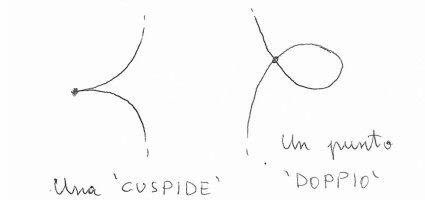
\includegraphics[width=20em]{punti-singolari.jpeg}
%\curvegraph{y**2 - x**2}{[-2:2]}{[-2:2]}
\begin{tikzpicture}[
    thick]
        \begin{axis}[
            xmin=-2, xmax=4,
            ymin=-5, ymax=5,
            axis x line = center,
            axis y line = center,
            xtick = \empty,
            ytick = \empty,
            xlabel = {$x$},
            ylabel = {$y$},
            legend style = {nodes=right},
            legend pos = north east,
            clip mode = individual,
            ]
            \addplot[red, samples=100, domain=-1:4] {sqrt(x^3+x^2)};
            \addplot[red, samples=100, domain=-1:4] {-sqrt(x^3+x^2)};
        \end{axis}
\end{tikzpicture}

\textit{Algebricamente}, un punto $p$ zero di $f$ è singolare se $\partial_{x_i}f(p)=0$ per $i=0,\ldots,n$ (ha il differenziale nullo). \notamargine{Se il campo ha caratteristica 0, notare che $\partial_{x_i}f(p) = 0$ per ogni $i$ implica $f(p)=0$ per il \href{https://it.wikipedia.org/wiki/Funzione_omogenea}{teorema di eulero} sulle funzioni omogenee.}


\section{Cubiche, forma di Weierstrass}
Nel caso speciale di $n=2$, $\chr \bbK = 0$ c'è un importante risultato di classificazione delle curve non singolari.
\notamargine{Una curva si dice non singolare se ogni suo punto è non singolare.}

Consideriamo curve descritte da
$$ zy^2= ax^3+bx^2z+cxz^2+dz^3 $$
 dove $ax^3+bx^2+cx+d$ è un polinomio senza radici multiple, detta \smallcaps{forma di weierstrass}. Allora è non singolare. Imponiamo infatti le tre equazioni:

%% ESERCIZIO: dimostrare che la forma di weierstrass è non singolare

$$ \left\{
\begin{matrix}
&3ax^2&+2bxz&+cz^2 & = & -\partial_{x}f & = 0 \\
&&yz& & = & \partial_{y}f / 2 &= 0 \\
y^2 &-bx^2&-2cx&-3dz^2 & = & \partial_{z}f& = 0 \\
ax^3&+bx^2z&+cxz^2&+dz^3& = & zy^2&
\end{matrix}
\right.$$

Dalla (2) abbiamo due casi:

\begin{itemize}
	\item Se $z=0$ allora (4) dà $x=0$ e dunque $y=0$ dalla (3), assurdo.
	\notamargine{ Siamo nel proiettivo: $x=y=z=0$ non è un punto!}

	\item Se $y = 0$, $z \neq 0$ allora (4) dà $q(x/z) = 0$ e (1) dà $q'(x/z) = 0$ (dove $q$ è il polinomio di coefficienti $a,b,c,d$). Ma allora $x/z$ sarebbe una radice multipla di $q$, assurdo.
	\notamargine{Infatti vale il criterio della derivata, cioè un polinomio $p$ ha radici multiple se e solo se $p$ e $p'$ hanno un fattore in comune.}
\end{itemize}

Viceversa, data una curva cubica non singolare, può essere descritta da un polinomio in forma di weierstrass. Algebricamente, per ogni polinomio omogeneo $f$ di grado 3 con differenziale mai nullo, esiste una $L \in \bbP GL_2(\bbK) $ tale che $f \circ L$ (che è ancora un polinomio omogeneo di grado 3) è in forma di Weierstrass.
\paragraph{IDEA}. Si dimostra che esiste un punto di flesso, e poi si considera una proiettività che manda il punto di flesso nel punto all'infinito. A quel punto, con pochi conti, si arriva alla forma di Weierstrass.
\notamargine{Un punto sulla cubica è di flesso se è un punto non singolare e la tangente ha ordine di contatto $>2$. Notare che nella forma di Weierstrass $(0:1:0)$ è un punto di flesso}

\section{Cubiche, struttura di gruppo}

Sia $\bbK$ algebricamente chiuso. Osserviamo che presi due punti $P,Q$ su una cubica $\gamma$ e tracciata la retta $r$ per $P,Q$, essa interseca $\gamma$ esattamente in un altro punto $R:=P * Q = Q*P$. \notamargine{Vedi il \href{https://en.wikipedia.org/wiki/B\%C3\%A9zout's_theorem}{Teorema di Bezòut}.}

Fissata un'origine $O \in \gamma$, si può dimostrare che l'operazione $(P,Q) \mapsto P \cdot Q = O*(P*Q)$ rende $\gamma$ un gruppo (banalmente) abeliano. Il cambio dell'origine dà luogo a un gruppo isomorfo. Infatti se $O,O'$ sono due origini diverse, detto $O'' = O*O'$, la mappa $P \mapsto O'' * P$ è l'isomorfismo cercato:
\notamargine{Solitamente, nella forma di weierstrass, si prende $O=(0:1:0)$, il punto all'infinito.}
$$ O'' * (P \cdot' Q) = O'' * O'*P*Q = O*P*Q $$
$$ (O''*P) \cdot (O''*Q) = (O*O'')*(P*O'')*Q = O'*O''*P*Q=O*P*Q$$

%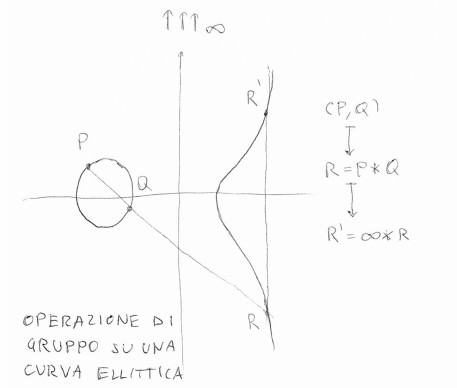
\includegraphics[width=16em]{gruppo-cubica.jpeg}

L'associatività è la proprietà più impegnativa da dimostrare. Vale la pena di notare che l'operazione è una funzione razionale delle coordinate dei punti.


\section{Gruppi algebrici}
\begin{definizione}[Gruppo algebrico]
  Si dice gruppo algebrico una varietà algebrica (ovvero un luogo di uno spazio affine o proiettivo definito da equazioni algebriche), dotata di una struttura di gruppo tale che l'operazione di gruppo sia un morfismo di varietà algebriche (equivalentemente, che sia espresso da funzioni razionali delle coordinate).
\end{definizione}

\paragraph{Esempi di gruppi algebrici}
Facciamo ora alcuni esempi di gruppi algebrici (li pensiamo tutti su $\bbC$):
\begin{itemize}
\item $\bbG_a$ come gruppo additivo (Si intende la retta affine $\bbA^1$ come varietà e come legge di gruppo $x \star y := x + y$). Possiamo osservare che è un gruppo algebrico non compatto di dimensione $1$
\item $\bbG_m$ come gruppo moltiplicativo (Si intende la retta affine tolto un punto $\bbA^1 \setminus \{ 0 \}$ come varietà [anche se in $\bbA^1$ non è un chiuso, lo è attraverso il morfismo con l'iperbole in $\bbA^2$], mentre la legge di gruppo è $x \star y := x y$). \\
  Esso si può anche interpretare come l'iperbole $xy=1$ (in $\bbA^2$) con legge di gruppo $(u_1, u_2) \star (t_1, t_2) = (u_1 t_1, u_2 t_2)$
\end{itemize}

Si può dimostrare che questi sono tutti i gruppi algebrici non compatti di dimensione $1$, mentre quelli compatti (sempre di dimensione $1$) sono tutte e sole le curve ellittiche (Infatti ``vengono'' dai tori).

\notamargine{Con dimensione intendiamo qui la dimensione come varietà olomorfa}

\notamargine{In dimensione superiore invece ce ne sono tanti, anche non commutativi, come $\GL_2 \bbC$}



\section{Funzioni ellittiche, curve ellittiche, reticoli}
C'è una stretta correlazione tra reticoli\notamargine{Per reticoli, dove non diversmaente specificato, intendermo reticoli di rango 2 nel piano complesso}, funzioni ellittiche, curve ellittiche.

Dato un reticolo $L$, saremo in grado di costruire una funzione meromorfa con gruppo dei periodi L detta $\wp_L$.
D'altronde, questa speciale funzione ellittica $\wp_L$ rispetta $\wp_L'(z)^2= f_L(\wp_L(z))$ per un opportuno polinomio di terzo grado $f_L$. Perciò, la funzione $\varphi_L: z \mapsto (\wp_L'(z), \wp_L(z) )$ parametrizza una cubica $E_L$.

\begin{diagram}
 \bbC & \rTo & E_L \\
 \dTo &  \ruTo    & \\
 \bbC/L & &  \\
\end{diagram}

\section{Moduli}
Vogliamo cercare ora uno 'spazio dei parametri' per i tori complessi. Conosciamo già una parametrizzazione ridondante: dato un reticolo discreto $L=\omega_1 \bbZ + \omega_2 \bbZ$ possiamo costruire il toro $\bbC / L$ ( e tutti i tori sono definiti così), con $\omega_1, \omega_2$ non paralleli (ossia $\omega_1/\omega_2$ non reale). Cerchiamo ora di eliminare la ridondanza della parametrizzazione, partendo da $\mathcal{A} = \{ (\omega_1, \omega_2) \in \bbC^2: \Im(\omega_1/\omega_2) \neq 0 \} $.

\begin{enumerate}
\item (orientazione) Anzitutto, a meno di scambiare $\omega_1, \omega_2$, possiamo supporre che $\Im(\omega_1/\omega_2) > 0$: infatti se fosse negativa, $\Im(\omega_2/\omega_1) = -\Im(\omega_1/\omega_2)  > 0$ sarebbe positiva.
\item (riscalamento) Se $\lambda \in \bbC^*$, allora $\bbC/\lambda L  \simeq \bbC/L$ tramite la mappa $z \mapsto \lambda z$ da $C/L$ in $C/\lambda L$. Dunque se $L= \omega_1\bbZ + \omega_2 \bbZ$ con $\Im(\omega_1/\omega_2) > 0$ possiamo considerare $\omega_2^{-1}L= \tau \bbZ + \bbZ $ con $\Im \tau > 0$. Ora il nostro spazio dei parametri perciò è $\mathcal{H} = \{ \tau \in \bbC: \Im \tau > 0 \} \simeq \mathcal{A} / \text{omotetie}$. Se $(\omega_1, \omega_2) \in \mathcal{A}$ indichiamo con $[\omega_1, \omega_2]$ la sua classe di equaivalenza a meno di omotetie, che ha un rappresentante privilegiato $[\omega_1/\omega_2, 1]$ in $\mathcal{H}$.
\item (cambio base) Se $M$ è una matrice 2x2 a coefficienti interi e $L=\omega_1\bbZ + \omega_2\bbZ$ è un reticolo, possiamo considerare il reticolo generato da $M[\omega_1, \omega_2]$ ($M \in End(\bbZ^2) \subset End(\bbC^2)$ agisce sulle coppie di complessi). Visto che le coppie di complessi sono a meno di omotetie, possiamo considerare $M,N \in End(\bbZ^2)$ equivalenti se esiste $\lambda \in \bbC^*$ tale che $\lambda M = N$. Il gruppo delle matrici invertibili a meno di scalari si chiama $\bbP GL_2(\bbZ)$. \notamargine{In realtà, visto che $M,N$ sono a coefficienti interi, $\lambda$ deve essere razionale.} Se $M \in \bbP GL_2(\bbZ)$, allora $M[\omega_1,\omega_2]$ è equivalente a $[\omega_1,\omega_2]$, perciò lo spazio dei parametri ora è $(\mathcal{A}/\text{omotetie})/\bbP GL_2(\bbZ)$.
\item (parametrizzazione esplicita) Così come per ogni classe di equivalenza $[\omega_1, \omega_2]$ a meno di omotetie abbiamo scelto un rappresentante privilegiato $[\tau,1]$, così scegliamo per ogni matrice $[M] \in \bbP GL_2(\bbZ)$ a meno di omotetie un rappresentante privilegiato in $SL_2(\bbQ)$. Infatti $[M*M'] = \mathrm{ Id} $ significa che esiste $\lambda \in \bbC^*$ tale che
$[M]*[M'] = \lambda \mathrm{Id} $. In particolare $\mathrm{det } M$ è invertibile, perciò possiamo scegliere $(\mathrm{det }M)^{-1}M$ equivalente a $M$ e condeterminante 1 ( e ha coefficienti in $\bbQ$). Se prendiamo ora $M \in SL_2(\bbQ)$ di coefficienti $a,b,c,d$ e lo facciamo agire su $[\tau,1]$ otteniamo $\displaystyle [a\tau+b,c\tau+d]= \left [ \frac{a\tau+b}{c \tau + d}, 1 \right ] $ .\notamargine{e si può verificare che  $\frac{a\tau+b}{c \tau + d}$ ha ancora parte immaginaria positiva.} Perciò $SL_2(\bbQ)$ agisce su $\mathcal{H}$ tramite $ M( \tau) = \frac{a \tau+b}{c\tau+d} $, e il nostro spazio dei parametri diventa infine $\mathcal{H} / SL_2(\bbQ)$.
\end{enumerate}

Dimostreremo nelle prossime lezioni che questa parametrizzazione non è più ridondante: se due tori hanno parametri diversi, allora \textit{non} sono biolomorfi. Questo seguirà dalla classificazione esplicita delle funzioni olomorfe tra tori (vedi lezione sulle isogenie).
